\documentclass[14pt]{extbook}
\usepackage{multicol, enumerate, enumitem, hyperref, color, soul, setspace, parskip, fancyhdr} %General Packages
\usepackage{amssymb, amsthm, amsmath, bbm, latexsym, units, mathtools} %Math Packages
\everymath{\displaystyle} %All math in Display Style
% Packages with additional options
\usepackage[headsep=0.5cm,headheight=12pt, left=1 in,right= 1 in,top= 1 in,bottom= 1 in]{geometry}
\usepackage[usenames,dvipsnames]{xcolor}
\usepackage{dashrule}  % Package to use the command below to create lines between items
\newcommand{\litem}[1]{\item#1\hspace*{-1cm}\rule{\textwidth}{0.4pt}}
\pagestyle{fancy}
\lhead{Progress Quiz 10}
\chead{}
\rhead{Version B}
\lfoot{6232-9639}
\cfoot{}
\rfoot{Fall 2020}
\begin{document}

\begin{enumerate}
\litem{
Solve the radical equation below. Then, choose the interval(s) that the solution(s) belongs to.\[ \sqrt{-24 x^2 - 18} - \sqrt{-62 x} = 0 \]\begin{enumerate}[label=\Alph*.]
\item \( \text{All solutions lead to invalid or complex values in the equation.} \)
\item \( x_1 \in [-0.31, 1.95] \text{ and } x_2 \in [0.25,10.25] \)
\item \( x \in [1.66,2.4] \)
\item \( x \in [-0.31,1.95] \)
\item \( x_1 \in [-1.06, 0.31] \text{ and } x_2 \in [-3.25,1.75] \)

\end{enumerate} }
\litem{
Solve the radical equation below. Then, choose the interval(s) that the solution(s) belongs to.\[ \sqrt{-81 x^2 - 21} - \sqrt{90 x} = 0 \]\begin{enumerate}[label=\Alph*.]
\item \( x \in [-1.3,-0.42] \)
\item \( x \in [-0.66,0.15] \)
\item \( x_1 \in [0, 1.5] \text{ and } x_2 \in [0.06,1.03] \)
\item \( x_1 \in [-1.3, -0.42] \text{ and } x_2 \in [-0.76,-0.27] \)
\item \( \text{All solutions lead to invalid or complex values in the equation.} \)

\end{enumerate} }
\litem{
Choose the graph of the equation below.\[ f(x) = \sqrt[3]{x + 8} + 6 \]\begin{enumerate}[label=\Alph*.]
\begin{multicols}{2}\item 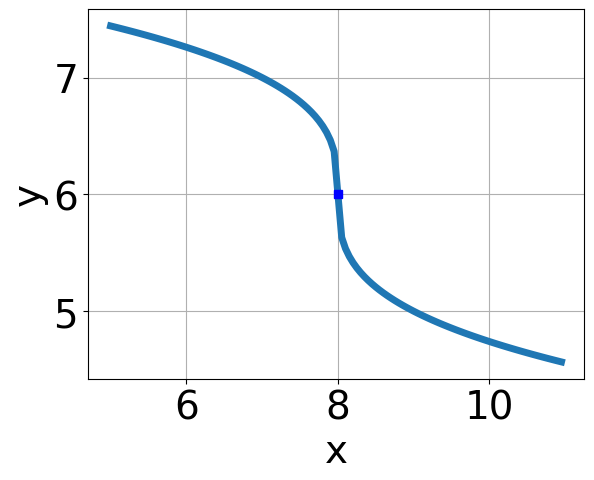
\includegraphics[width = 0.3\textwidth]{../Figures/radicalEquationToGraphCopyAB.png}\item 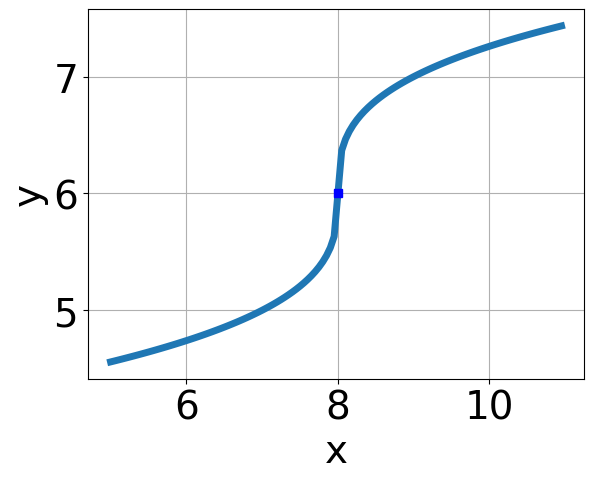
\includegraphics[width = 0.3\textwidth]{../Figures/radicalEquationToGraphCopyBB.png}\item 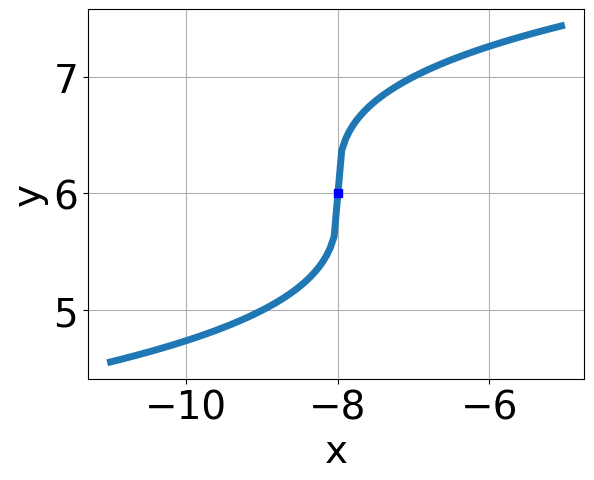
\includegraphics[width = 0.3\textwidth]{../Figures/radicalEquationToGraphCopyCB.png}\item 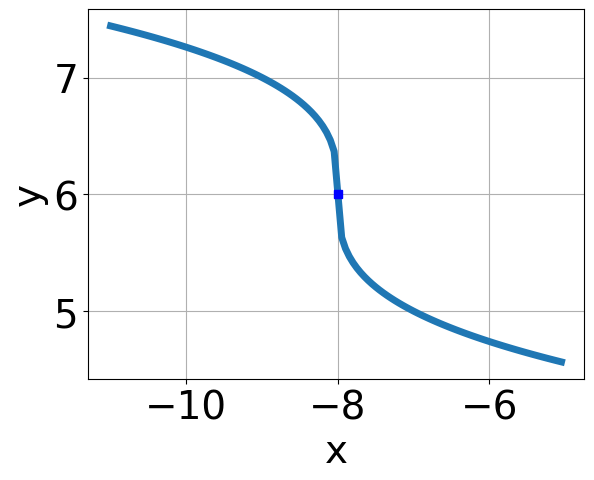
\includegraphics[width = 0.3\textwidth]{../Figures/radicalEquationToGraphCopyDB.png}\end{multicols}\item None of the above.
\end{enumerate} }
\litem{
What is the domain of the function below?\[ f(x) = \sqrt[7]{4 x - 3} \]\begin{enumerate}[label=\Alph*.]
\item \( (-\infty, \infty) \)
\item \( \text{The domain is } [a, \infty), \text{   where } a \in [1.07, 1.82] \)
\item \( \text{The domain is } (-\infty, a], \text{   where } a \in [-0.11, 1.07] \)
\item \( \text{The domain is } [a, \infty), \text{   where } a \in [-0.07, 0.92] \)
\item \( \text{The domain is } (-\infty, a], \text{   where } a \in [0.79, 3.54] \)

\end{enumerate} }
\litem{
Choose the graph of the equation below.\[ f(x) = - \sqrt{x + 12} - 6 \]\begin{enumerate}[label=\Alph*.]
\begin{multicols}{2}\item 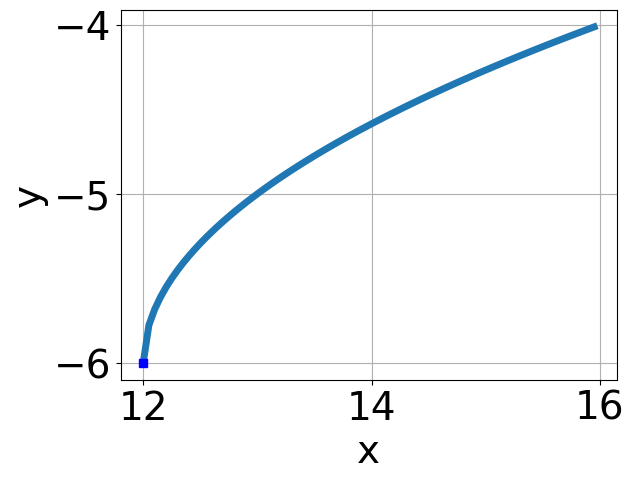
\includegraphics[width = 0.3\textwidth]{../Figures/radicalEquationToGraphAB.png}\item 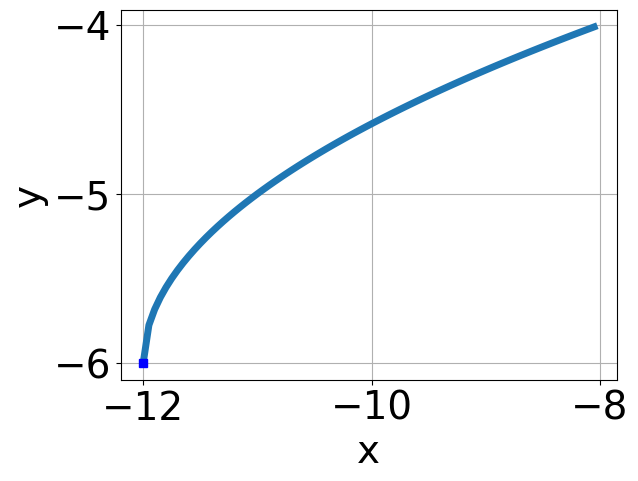
\includegraphics[width = 0.3\textwidth]{../Figures/radicalEquationToGraphBB.png}\item 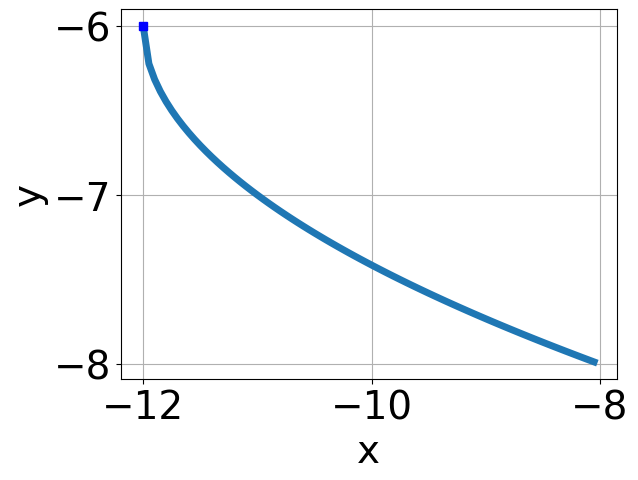
\includegraphics[width = 0.3\textwidth]{../Figures/radicalEquationToGraphCB.png}\item 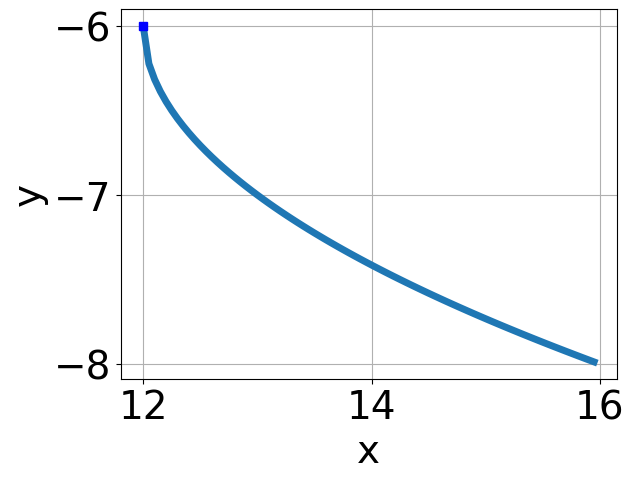
\includegraphics[width = 0.3\textwidth]{../Figures/radicalEquationToGraphDB.png}\end{multicols}\item None of the above.
\end{enumerate} }
\litem{
Choose the equation of the function graphed below.
\begin{center}
    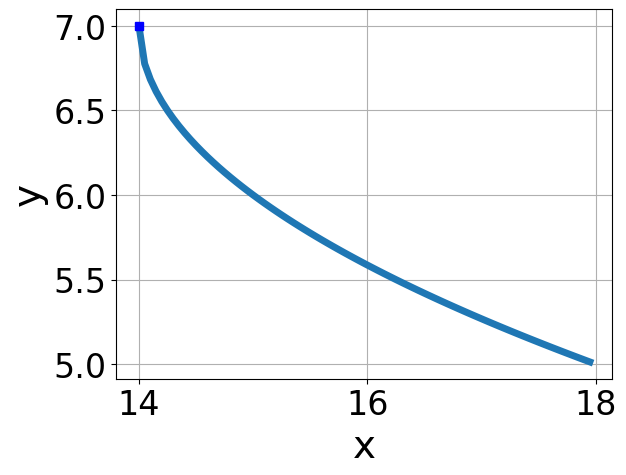
\includegraphics[width=0.5\textwidth]{../Figures/radicalGraphToEquationB.png}
\end{center}
\begin{enumerate}[label=\Alph*.]
\item \( f(x) = \sqrt{x + 14} + 7 \)
\item \( f(x) = - \sqrt{x + 14} + 7 \)
\item \( f(x) = - \sqrt{x - 14} + 7 \)
\item \( f(x) = \sqrt{x - 14} + 7 \)
\item \( \text{None of the above} \)

\end{enumerate} }
\litem{
Solve the radical equation below. Then, choose the interval(s) that the solution(s) belongs to.\[ \sqrt{9 x - 8} - \sqrt{4 x - 3} = 0 \]\begin{enumerate}[label=\Alph*.]
\item \( \text{All solutions lead to invalid or complex values in the equation.} \)
\item \( x \in [2.15,2.39] \)
\item \( x_1 \in [0.68, 0.83] \text{ and } x_2 \in [0.6,0.89] \)
\item \( x \in [0.97,1.04] \)
\item \( x_1 \in [0.8, 0.93] \text{ and } x_2 \in [0.91,1.31] \)

\end{enumerate} }
\litem{
Solve the radical equation below. Then, choose the interval(s) that the solution(s) belongs to.\[ \sqrt{-9 x - 2} - \sqrt{9 x - 6} = 0 \]\begin{enumerate}[label=\Alph*.]
\item \( \text{All solutions lead to invalid or complex values in the equation.} \)
\item \( x \in [-0.55,-0.44] \)
\item \( x_1 \in [-0.34, -0.12] \text{ and } x_2 \in [-0.22,0.41] \)
\item \( x \in [0.19,0.24] \)
\item \( x_1 \in [-0.34, -0.12] \text{ and } x_2 \in [0.35,1] \)

\end{enumerate} }
\litem{
What is the domain of the function below?\[ f(x) = \sqrt[4]{3 x + 7} \]\begin{enumerate}[label=\Alph*.]
\item \( [a, \infty), \text{where } a \in [-1.37, 1.2] \)
\item \( (-\infty, \infty) \)
\item \( (-\infty, a], \text{where } a \in [-1.57, -0.12] \)
\item \( (-\infty, a], \text{where } a \in [-2.57, -2.32] \)
\item \( [a, \infty), \text{ where } a \in [-2.34, -1.39] \)

\end{enumerate} }
\litem{
Choose the equation of the function graphed below.
\begin{center}
    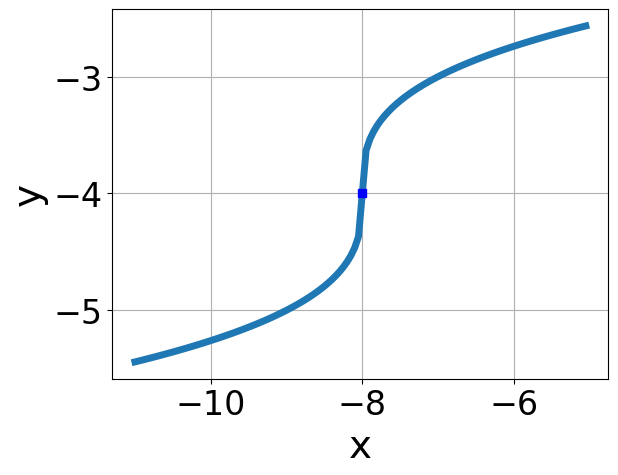
\includegraphics[width=0.5\textwidth]{../Figures/radicalGraphToEquationCopyB.png}
\end{center}
\begin{enumerate}[label=\Alph*.]
\item \( f(x) = - \sqrt[3]{x + 8} - 4 \)
\item \( f(x) = \sqrt[3]{x + 8} - 4 \)
\item \( f(x) = \sqrt[3]{x - 8} - 4 \)
\item \( f(x) = - \sqrt[3]{x - 8} - 4 \)
\item \( \text{None of the above} \)

\end{enumerate} }
\end{enumerate}

\end{document}